\subsection{Differentiable}
Now that we have introduced the derivative
of a function at a point, we can begin to use the adjective \dfont{differentiable}.

\begin{definition}{Differentiable at a Point}{DifferentiablePoint}
A function $f$ is
differentiable at point $a$ if $f'(a)$ exists.
\end{definition}

\begin{definition}{Differentiable on an Interval}{Differentiable}
A function $f$ is differentiable on an open interval if it is differentiable at every point in the interval.
\end{definition}

Sometimes one encounters a point in the domain of a function $y=f(x)$ where
there is {\bf no derivative}, because there is no tangent line.  In order
for the notion of the tangent line at a point to make sense, the curve must
be ``smooth'' at that point.  This means that if you imagine a particle
traveling at some steady speed along the curve, then the particle does not
experience an abrupt change of direction.  There are two types of
situations you should be aware of---corners and cusps---where there's a
sudden change of direction and hence no derivative.

\begin{example}{Derivative of the Absolute Value}{DerivativeAbsoluteValue}
Discuss the derivative of the absolute value function $y=f(x)=|x|$.
\end{example}

\begin{solution} 
If $x$ is positive, then this is the function $y=x$, whose derivative is
the constant 1.  (Recall that when $y=f(x)=mx+b$, the derivative is the
slope $m$.)  If $x$ is negative, then we're dealing with the function $y=-x$,
whose derivative is the constant $-1$.  If $x=0$, then the function has
a corner, i.e., there is no tangent line.  A tangent line 
would have to point in the direction of the curve---but there are {\it
two} directions of the curve that come together at the origin.

$$\includegraphics[width=2.5in]{images/absvalue}$$

We can summarize this as
$$ 
y'=\left\{\begin{array}{rl}
1, & \mbox{if $x>0$,}\\
-1, & \mbox{if $x<0$,}\\
\hbox{undefined,} & \mbox{if $x=0$.}\\
\end{array}\right.
$$
In particular, the absolute value function $f(x)=|x|$ is \ifont{not} differentiable at $x=0$.
\end{solution}

We note that the following theorem can be proved using limits.

\begin{theorem}{Differentiable implies Continuity}{DifferentiableImpliesContinuity}
If $f$ is differentiable at $a$, then $f$ is continuous at $a$.
\end{theorem}
\begin{proof}
Suppose that $f$ is differentiable at $a.$ That is,%
\begin{equation*}
	f^{\prime }\left( a\right) =\lim_{h\rightarrow 0}\frac{f\left( a+h\right)
		-f\left( a\right) }{h}
\end{equation*}%
exists. At this stage, we find it convenient to write this limit in an
alternative form so that its connection with continuity can become more
easily seen. If we let $x=a+h,$ then $h=x-a.$ Furthermore, $h\rightarrow 0$
is equivalent to $x\rightarrow a.$ So,%
\begin{equation*}
	f^{\prime }\left( a\right) =\lim_{x\rightarrow a}\frac{f\left( x\right)
		-f\left( a\right) }{x-a}.
\end{equation*}%
(This alternative formulation of the derivative is also standard. We will
use it whenever we find it convenient to do so. You should get familiar with
it.) Continuity at $a$ can now be proved as follows:%
\begin{eqnarray*}
	\lim_{x\rightarrow a}f\left( x\right) &=&\lim_{x\rightarrow a}\left( \frac{%
		f\left( x\right) -f\left( a\right) }{x-a}\cdot \left( x-a\right) +f\left(
	a\right) \right) \\
	&=&\lim_{x\rightarrow a}\frac{f\left( x\right) -f\left( a\right) }{x-a}\cdot
	\lim_{x\rightarrow a}\left( x-a\right) +\lim_{x\rightarrow a}f\left( a\right)
	\\
	&=&f^{\prime }\left( a\right) \cdot \left( a-a\right) +f\left( a\right) \\
	&=&f\left( a\right).
\end{eqnarray*}
\end{proof}

However, if $f$ is continuous at $a$ it is \ifont{not} necessarily
true that $f$ is differentiable at $a$.  For example, it was shown
that $f(x)=|x|$ is not differentiable at $x=0$ in the previous
example, however, one can observe that $f(x)=|x|$ is continuous
everywhere.

\begin{example}{Derivative of $\ds y=x^{2/3}$}{Derivative}
Discuss the derivative of the function $\ds y=x^{2/3}$, shown in
Figure~\ref{fig:cusp}. 
\end{example}

\begin{solution} 
We will later see how to compute this
derivative; for now we use the fact that $\ds
y'=(2/3)x^{-1/3}$. Visually this looks much like the absolute value
function, but it technically has a cusp, not a corner. The absolute
value function has no tangent line at 0 because there are (at least)
two obvious contenders---the tangent line of the left side of the
curve and the tangent line of the right side.
The function $\ds y=x^{2/3}$ does not have a tangent line at 0, but
unlike the absolute value function it can be said to have a single
direction: as we approach 0 from either side the tangent line becomes
closer and closer to a vertical line; the curve is vertical at 0. But
as before, if you imagine traveling along the curve, an abrupt change
in direction is required at 0: a full 180 degree turn.  
\end{solution}

\figure
\centerline{\vbox{\beginpicture
\normalgraphs
%\ninepoint
\setcoordinatesystem units <2truecm,2truecm>
\setplotarea x from -2 to 2, y from 0 to 1.6
\axis left shiftedto x=0 ticks numbered from 0 to 1 by 1 /
\axis bottom ticks numbered from -2 to 2 by 1 /
\setquadratic
\plot -2.000 1.587 -1.933 1.552 -1.867 1.516 -1.800 1.480 -1.733 1.443 
-1.667 1.406 -1.600 1.368 -1.533 1.330 -1.467 1.291 -1.400 1.251 
-1.333 1.211 -1.267 1.171 -1.200 1.129 -1.133 1.087 -1.067 1.044 
-1.000 1.000 -0.933 0.955 -0.867 0.909 -0.800 0.862 -0.733 0.813 
-0.667 0.763 -0.600 0.711 -0.533 0.658 -0.467 0.602 -0.400 0.543 
-0.333 0.481 -0.267 0.414 -0.200 0.342 -0.133 0.261 -0.067 0.164 
0.000 0.000 0.067 0.164 0.133 0.261 0.200 0.342 0.267 0.414 
0.333 0.481 0.400 0.543 0.467 0.602 0.533 0.658 0.600 0.711 
0.667 0.763 0.733 0.813 0.800 0.862 0.867 0.909 0.933 0.955 
1.000 1.000 1.067 1.044 1.133 1.087 1.200 1.129 1.267 1.171 
1.333 1.211 1.400 1.251 1.467 1.291 1.533 1.330 1.600 1.368 
1.667 1.406 1.733 1.443 1.800 1.480 1.867 1.516 1.933 1.552 
2.000 1.587   /
\endpicture}}
\caption{A cusp on $\ds x^{2/3}$. \label{fig:cusp}}
\endfigure

In practice we won't worry much about the distinction between these
examples; in both cases the function has a ``sharp point'' where there
is no tangent line and no derivative.